\chapter{Примеры задач}
\selectlanguage{russian}
\taskinit

В данном разделе приведены примеры задач, которые использовались на контрольных работах в МФТИ по курсу <<Защита информации>> в 2011--2014 годах.

Задачи приведены с ответами для самостоятельной проверки, но без решений.

\section{Математические основы}
\tasksection

\tasknumber Найдите общее количество и перечислите генераторы аддитивной циклической группы $\mathbb{Z}_{33}$ с операцией в виде сложения чисел по модулю 33.
\\*
\textbf{Ответ:} 20: [1, 2, 4, 5, 7, 8, 10, 13, 14, 16, 17, 19, 20, 23, 25, 26, 28, 29, 31, 32].
\\

\tasknumber Вычислить в поле Галуа $GF\left( {2^{5} } \right)$, $m\left( x \right) = x^{5} + x^{3} + x^{2} + x + 1$, следующее значение: $28 \times 29 + 23^2$. Многочлены заданы как десятичное представление двоичных коэффициентов, свободный член многочлена соответствует самому младшему биту двоичного представления. В ответе привести в десятичном представлении результаты умножения, возведения в степень и сложения.
\\*
\textbf{Ответ:} 27; 28; 7.
\\

\tasknumber Вычислить в поле Галуа $GF\left( {27 } \right)$, $m\left( x \right) = x^{3} + x^{2} + x + 2$, следующее значение: $26 \times 11 + 25^2$. Многочлены заданы как десятичное представление троичных коэффициентов, свободный член многочлена соответствует самому младшему биту троичного представления. В ответе привести в десятичном представлении результаты умножения, возведения в степень и сложения.
\\*
\textbf{Ответ:} 10; 5; 12.
\\

\tasknumber Используя алгоритм быстрого возведения в степень (с помощью разложения показателя степени по степеням двойки по схеме <<слева направо>>) вычислить ${175}^{235} \mod {257}$.
\\*
\textbf{Ответ:} 3.
\\

\section{Общие определения и теория}
\tasksection

\tasknumber Рассмотрим множество паролей, состоящих из 12 строчных и заглавных латинских букв, а также цифр.
\begin{itemize}
\item каков размер этого множества?
\item сколько времени потребуется на взлом шифротекста, зашифрованного данным паролем, если предположить, что во взломе участвуют все компьютеры мира (7~млрд.), а средний компьютер перебирает $10^5$ паролей в секунду?
\item каковы затраты электроэнергии в денежном эквиваленте, если средний компьютер потребляет мощность 400~Вт, а стоимость 1~кВт$\times$час составляет 2~рубля?
\end{itemize}
\\*
\textbf{Ответ:} паролей $3,226\times 10^{21}$; на перебор нужно $4,609\times 10^{6}$ секунд ($\approx 21$ день); затраты $7,169\times 10^{12}$ руб.
\\

\tasknumber Источник открытого текста характеризуется случайной величиной $X$, принимающей два значения $x_1$ и $x_2$ с вероятностями $p \left( x = x_1 \right) = 1/5$ и $p \left( x = x_2 \right) = 4/5$ соответственно. Источник ключей характеризуется случайной величиной $Z$, независимой от величины $X$,  принимающей два значения $z_1$ и $z_2$ с вероятностями $p \left( z = z_1 \right) = 1/6$ и $p \left( z = z_2 \right) = 5/6$ соответственно. Функция шифрования $E_{z} \left( x \right)$ задаётся следующими правилами: $\left( x_1, z_1 \right) \to y_1$, $\left( x_1, z_2 \right) \to y_2$, $\left( x_2, z_1 \right) \to y_2$, $\left( x_2, z_2 \right) \to y_1$.
\begin{enumerate}
	\item Найдите собственную информацию каждого из сообщений открытого текста в битах.
	\item Найдите энтропию источника сообщений, источника ключей и шифротекста в битах.
	\item Найдите взаимную информацию открытого текста и ключа в битах.
	\item Найдите взаимную информацию открытого текста и шифротекста в битах.
	\item Найдите взаимную информацию ключа и шифротекста в битах.
	\item Найдите апостериорное распределение вероятностей открытого текста для обоих вариантов перехваченных злоумышленником шифротекстов $y_1$ и $y_2$. Используя вычисленные значения, определите, является ли данная шифросистема абсолютно надёжной. Если нет, то что в данной криптосистеме необходимо поменять? Покажите, что апостериорные вероятности после доработки будут удовлетворять необходимым требованиям абсолютно надёжной криптосистемы.
\end{enumerate}
\\
\textbf{Ответ:} \begin{itemize}
	\item $I \left( x_1 \right) = \log_2 5 = 2,322$ бит; $I \left( x_1 \right) = \log_2 5/4 = 0,322$ бит;
	\item $H \left( X \right) = 0,722$ бит; $H \left( Z \right) = 0,650$ бит; $H \left( Y \right) = 0,881$ бит;
	\item $I \left( X ; Z \right) = 0$ бит; $I \left( X; Y \right) = 0,231$ бит; $I \left( Y; Z \right) = 0,159$ бит;
	\item $p \left( x_1 | y_1 \right) = 1/21$; $p \left( x_1 | y_2 \right) = 20/21$; $p \left( x_2 | y_1 \right) = 5/9$; $p \left( x_2 | y_2 \right) = 4/9$; не является.
\end{itemize}

\section{КСГПСЧ и потоковые шифры}
\tasksection

\tasknumber Привести следующие два элемента последовательности, сформированной линейным конгруэнтным методом, если предыдущие 3 элемента последовательности такие: 348, 65, 139, а все вычисления выполняются в поле $\mathbb{F}_{499}$.
\\*
\textbf{Ответ:} 266, 194.
\\

\tasknumber Приведите \textit{предыдущие} 5 бит выхода генератора псевдослучайной последовательности, основанного на регистре сдвига с линейной обратной связью, если известно, что характеристический полином регистра — $m\left(x\right)=x^{5} + x^{3} + 1$ (см. рис.), а дальнейшая последовательность такова: $1,1,0,1,0,1$.
\begin{center}
	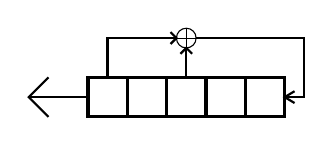
\begin{tikzpicture}[scale=0.05]
		\draw[black,very thick] (30,30) -- (30,40) -- (40,40) -- (40,30) -- (30,30) -- (30,40);
		\draw[black,thick] (35,40) -- (35,50) -- (35,50) -- (37.5,50);
		\draw[black,very thick] (40,30) -- (40,40) -- (50,40) -- (50,30) -- (40,30) -- (40,40);
		\draw[black,very thick] (50,30) -- (50,40) -- (60,40) -- (60,30) -- (50,30) -- (50,40);
		\draw[black,thick] (55,40) -- (55,47.5);
		\draw[black,thick] (53.5,46) -- (55,47.5) -- (56.5,46);
		\draw[black,thick] (37.5,50) -- (52.5,50);
		\draw[black,thick] (51,51.5) -- (52.5,50) -- (51,48.5);
		\draw (55,50) circle [radius=2.5];
		\draw[black] (52.5,50) -- (57.5,50);
		\draw[black] (55,47.5) -- (55,52.5);
		\draw[black,very thick] (60,30) -- (60,40) -- (70,40) -- (70,30) -- (60,30) -- (60,40);
		\draw[black,very thick] (70,30) -- (70,40) -- (80,40) -- (80,30) -- (70,30) -- (70,40);
		\draw[black,thick] (57.5,50) -- (85,50) -- (85,35) -- (80,35);
		\draw[black,thick] (82.5,36.5) -- (80,35) -- (82.5,33.5);
		\draw[black,thick] (30,35) -- (15,35);
		\draw[black,thick] (20,30) -- (15,35) -- (20,40);
	\end{tikzpicture}
\end{center}
\\*
\textbf{Ответ:} $0, 1, 1, 0, 1$.
\\

\tasknumber Укажите характеристический полином и приведите следующие 5 бит выхода генератора псевдослучайной последовательности, основанного на регистре сдвига с линейной обратной связью, если известно, что степень характеристического полинома регистра -- $m\left(x\right)$ -- равна 5, а предыдущая последовательность такова: $0,1,0,0,1,1,0,0,0,0,1$. Порядок бит в последовательности соответствует порядку их генерации РСЛОС.
\\*
\textbf{Ответ:} Полином $m \left( x \right) = x^{5} + x^{4} + x^{3} + x^{2} + 1$. Дальнейшая последовательность: $0,1,1,0,1$

\section{Псевдопростые числа}
\tasksection

\tasknumber Проверить, являются ли числа 73, 95 свидетелями простоты числа 111 по Ферма.
\\*
\textbf{Ответ:} да; нет.
\\

\tasknumber Проверить, являются ли числа 74, 448, 640, 660, 719 свидетелями простоты числа 793 по Миллеру.
\\*
\textbf{Ответ:} да; да; нет; нет; да.
\\

\section{Криптосистема RSA}
\tasksection

\tasknumber Зашифровать сообщение по схеме RSA. Открытый ключ: $n = 323$; $e = 245$. Сообщение: $m = 307$.
\\*
\textbf{Ответ:} $c = 86$.
\\

\tasknumber Расшифровать сообщение по схеме RSA. Для генерации пары открытого и секретного ключа использовались числа: $p = 13$; $q = 17$. Открытая экспонента: $e = 91$. Зашифрованное сообщение: $c = 196$.
\\*
\textbf{Ответ:} $d = 19$; $m = 66$.
\\

\tasknumber Расшифровать сообщение по схеме RSA. Открытый ключ: $n = 85$; $e = 15$. Зашифрованное сообщение: $c = 32$.
\\*
\textbf{Ответ:} $p = 5$; $q = 17$; $d = 47$; $m = 8$.
\\

\tasknumber Подписать сообщение по схеме RSA.  Закрытый ключ: $n = 437$; $d = 181$. Сообщение: $m = 84$.
\\*
\textbf{Ответ:} $s = 122$.
\\

\tasknumber Подписать сообщение по схеме RSA. Открытый ключ: $n = 253$; $e = 119$. Сообщение: $m = 193$.
\\*
\textbf{Ответ:} $n = 11 \cdot 23$; $d = 119$; $s = 2$.

\section{Криптосистема Эль-Гамаля}
\tasksection

\tasknumber Зашифровать сообщение по схеме Эль-Гамаля. Открытый ключ: $p = 29$; $g = 10$; $y = 8$. Секретный ключ: $x = 5$. Сообщение: $M = 4$. Использовать следующий случайный параметр для шифрования: $k = 5$.
\\*
\textbf{Ответ:} $c = (a; b) = (8; 21)$.
\\

\tasknumber Расшифровать сообщение по схеме Эль-Гамаля. Открытый ключ: $p = 23$; $g = 5$; $y = 9$. Секретный ключ: $x = 10$. Зашифрованное сообщение: $\left( 10, 18\right)$.
\\*
\textbf{Ответ:} $m = 4$.
\\

\tasknumber Расшифровать сообщение по схеме Эль-Гамаля. Открытый ключ: $p = 29$; $g = 15$; $y = 28$. Зашифрованное сообщение: $\left( 10, 23\right)$.
\\*
\textbf{Ответ:} $x = 14$; $m = 6$.
\\

\tasknumber Проверить подпись по схеме Эль-Гамаля. Открытый ключ: $p = 29$; $g = 14$; $y = 7$. Сообщение: $m = 7$. Подпись: $a = 19$;  $b = 19$.
\\*
\textbf{Ответ:} $12 = 12$.
\\

\tasknumber Подписать сообщение по схеме Эль-Гамаля. Открытый ключ: $p = 23$; $g = 20$; $y = 17$. Сообщение: $m = 4$. Использовать следующий случайный параметр для создания подписи: $k = 7$.
\\*
\textbf{Ответ:} $x = 19$; $s = (a; b) = (21; 19)$.
\\

\section{Эллиптические кривые}
\tasksection

\tasknumber Для точки A (8; 6) принадлежащей группе точек эллиптической кривой $y^2 = x^3 - 9x - 13$ над конечным полем $\mathbb{F}_{17}$ найти координаты точек $B = 2 \times A = A + A$ и $C = 3 \times A$ = A + A + A.
\\*
\textbf{Ответ:} $(3; 15)$, $(14; 15)$.
\\

\tasknumber Найти группу точек (перечислить все точки) эллиптической кривой $y^2 = x^3 - 2 x - 10$ над конечным полем $\mathbb{F}_{13}$.
\begin{itemize}
\item \textbf{Решение и ответ:}
\item Получение группы точек с помощью таблицы:\\
\begin{tabular}{|r|r|r|r|r|r|r|r|}
\hline
$x$ & $x^2$ & $x^3$ & $-2x$ & $-10$ & $y^2$ & $y_1$, $y_2$ & точки \\ 
\hline
$0$ & $0$ & $0$ & $-0$ & $-10$ & $3$ & $4$,$9$ &$(0; 4)$, $(0; 9)$ \\ 
$1$ & $1$ & $1$ & $-2$ & $-10$ & $2$ &  --- & --- \\ 
$2$ & $4$ & $8$ & $-4$ & $-10$ & $7$ &  --- & --- \\ 
$3$ & $9$ & $1$ & $-6$ & $-10$ & $11$ &  --- & --- \\ 
$4$ & $3$ & $12$ & $-8$ & $-10$ & $7$ &  --- & --- \\ 
$5$ & $12$ & $8$ & $-10$ & $-10$ & $1$ & $1$,$12$ &$(5; 1)$, $(5; 12)$ \\ 
$6$ & $10$ & $8$ & $-12$ & $-10$ & $12$ & $5$,$8$ &$(6; 5)$, $(6; 8)$ \\ 
$7$ & $10$ & $5$ & $-1$ & $-10$ & $7$ &  --- & --- \\ 
$8$ & $12$ & $5$ & $-3$ & $-10$ & $5$ &  --- & --- \\ 
$9$ & $3$ & $1$ & $-5$ & $-10$ & $12$ & $5$,$8$ &$(9; 5)$, $(9; 8)$ \\ 
$10$ & $9$ & $12$ & $-7$ & $-10$ & $8$ &  --- & --- \\ 
$11$ & $4$ & $5$ & $-9$ & $-10$ & $12$ & $5$,$8$ &$(11; 5)$, $(11; 8)$ \\ 
$12$ & $1$ & $12$ & $-11$ & $-10$ & $4$ & $2$,$11$ &$(12; 2)$, $(12; 11)$ \\ 
\hline
\end{tabular}
\item Точки эллиптической кривой: [(0; 4), (0; 9), (5; 1), (5; 12), (6; 5), (6; 8), (9; 5), (9; 8), (11; 5), (11; 8), (12; 2), (12; 11), 0]
\item Размер группы точек: $13$
\end{itemize}
\\

\tasknumber Для точки $\left(6; 9\right)$ определить, является ли она генератором всей группы точек кривой $y^2 = x^3 - 10 x - 7$ над конечным полем $\mathbb{F}_{17}$, либо подгруппы. Перечислить точки генерируемой подгруппы (группы).
\\*
\textbf{Ответ:} точка $\left(6; 9\right)$ — генератор подгруппы размера 4: [(6; 9), (4; 0), (6; 8), 0]
\\

\tasknumber Вычислить электронную подпись сообщения $m=5$ по схеме ГОСТ Р 34.10-2012. Кривая $y^2 = x^3 - 2 x - 10$ над конечным полем $\mathbb{F}_{13}$. В качестве генератора используется точка G$\left(6; 8\right)$. Открытый ключ отправителя сообщения Q$\left(11; 8\right)$. Для генерации ЭП использовать случайный параметр $k=4$.
\begin{itemize}
\item \textbf{Решение и ответ:} используя формулу $Q = d \times G$, перебором находим, что $d = 3$.
\item $C = k \times G = 4 \times \left(6; 8\right) = \left(9; 5\right)$.
\item $s = ( x_c d + k m ) \bmod n = ( 9 \cdot 3 + 4 \cdot 5 ) \bmod 13 = 8$.
\item Подпись: $(x_c, s) = (9, 8)$.
\end{itemize}

\section{Протоколы распространение ключей}
\tasksection

\tasknumber Алиса и Боб участвуют в группе распределения ключей по схеме Блома с модулем $p = 11$. Алисе выдан идентификатор $\overrightarrow{(5; 7)}$ и соответствующий ему закрытый ключ $\overrightarrow{(5; 8)}$. Вычислите общий сеансовый ключ Алисы и Боба, если открытый ключ Боба $\overrightarrow{(4; 3)}$. Найдите секретную матрицу доверенного центра, если известно, что закрытый ключ Боба -- $\overrightarrow{(1; 4)}$.
\\*
\textbf{Ответ:} $s = 0$. $\left( {\begin{array}{*{20}c}
   7 & 2  \\
   2 & 6  \\
\end{array}} \right)$ -- секретная матрица доверенного центра.
\\

\tasknumber Сгенерировать секретный сеансовый ключ для Алисы и Боба по протоколу Диффи~---~Хеллмана\index{протокол!Диффи~---~Хеллмана}. Общие параметры схемы: генератор 14 и модуль 17. Открытые ключи Алисы и Боба равны 8 и 5 соответственно.
\begin{itemize}
\item \textbf{Решение и ответ:}
\item Закрытый ключ Алисы: $a = \log_{g} A \bmod p = \log_{14} 8 \bmod 17 = 10$
\item Закрытый ключ Боба: $b = \log_{g} B \bmod p = \log_{14} 5 \bmod 17 = 13$
\item Генерация Алисой: $s = {B}^{a} \bmod p  = {5}^{10} \bmod 17 = 9$
\item Генерация Бобом: $s = {A}^{b} \bmod p  = {8}^{13} \bmod 17 = 9$
\end{itemize}

\section{Разделение секрета}
\tasksection

\tasknumber При разделении секрета по $(k, n)$-пороговой векторной схеме\index{схема!векторная} (схеме Блэкли\index{схема!Блэкли}) с модулем $p = 11$ получены 4 следа: $\left( {8,1,4} \right)$, $\left( {9,8,10} \right)$, $\left( {4,2,1} \right)$, $\left( {4,7,5} \right)$. Восстановите исходную точку и секрет, если известно, что это первая координата (x) точки.
\\*
\textbf{Ответ:} $M = 4$
\\

\tasknumber Секрет был разделён по $(3, n)$-пороговой схеме Шамира\index{схема!Шамира} с модулем $p=11$. Известны четыре следа -- $\left( {3,9} \right)$, $\left( {4,9} \right)$, $\left( {5,10} \right)$, $\left( {6,1} \right)$. Восстановить оптимальным способом исходный многочлен и секрет.
\\*
\textbf{Ответ:} Исходный многочлен: $F\left( x \right) = ax^2  + bx + M = 6x^2  + 2x + 4$. Секретом является последний свободный многочлен $M = 4$.
\\

\tasknumber Используя эллиптическую кривую $y^2 = x^3 - 1x - 7$ над конечным полем $\mathbb{F}_{11}$, генератор $G(0; 2)$ и открытый ключ Боба $K_R(10; 9)$, Алиса сгенерировала разделяемый секрет (по схеме ECIES\index{схема!ECIES}) $S=P_x$ для последующего использования в качестве ключа шифрования и передала Бобу соответствующий секрету след $R(9; 8)$. Найдите секрет $S$, если закрытый ключ Боба $k_B = 6$.
\\*
\textbf{Ответ:} $P_x = 5$
